\chapter{Introduction}
\label{chap-introduction}
\begin{ChapAbstract}
% In this chapter, overview of recent developments of machine learning as well as deep learning in Computer Vision and their applications to conduct medical image analysis are represented. Segmentation is discussed in more details to indicate our motivations and objectives in this thesis. Besides, in this chapter, we also provide an overview of our thesis's structure.
In this chapter, an overview of recent developments of machine learning as well as deep learning in Computer Vision and their applications to conduct medical image analysis are represented. Classification, object detection together with segmentation are discussed in more details to indicate our motivations and objectives in this thesis. Besides, in this chapter, we also provide an overview of our thesis's structure.

\end{ChapAbstract}

\section{Overview}
\subsection{Deep Learning in Computer Vision}

Computer Vision, besides other areas such as natural language processing, machine translation, ... is one of the most important branches in Artificial Intelligence. Some struggling problems, for example object detection or object segmentation, have been remaining one of the most challenging ones in this area. 

To solve these problems, in the early stage, many feature extractors \cite{SIFTFeatures,SURFFeatures} from image processing and signal processing techniques have been proposed to create more discriminate features than the original representations, like RGB image. K-means algorithm \cite{kmean} or K-nearest neighbors \cite{knearestneighbor} are then built on top these extracted features to further perform main tasks in Computer Vision such as object detection, image retrieval, image matching, etc. However, the performance of these approaches are not sufficient enough for the real-life application. The support vector machines \cite{SVM} can create finer boundary in high-dimensional space from these extracted features compared to the mentioned approaches. One big drawback of the SVMs \cite{SVM} family is that it still depends on the handcrafted features, such as kernel functions, from human experts, that could limit the searching ability of algorithm in the high-dimensional space.    

With the increasing availability of sensors including cameras, microphone, ..., a large a mount of data have been recorded every day. To turn these data to useful information, they should be organized in the way that both human and computer can understand. Therefore, a large number of standardized data have been created by the effort of both academic section and industry company. These large amount of data, as well as the development of the graphical processing units, are main factors pushing the machine learning, especially deep learning, to a new peak. There are some famous dataset that are often considered as baseline data to build up an algorithm in some areas such as ImageNet \cite{ImageNet} for object recognition, Pascal Visual Object Classes (PASCAL VOC) \cite{PASCALVOCDataset} and MS Common Object in Context (MSCOCO) \cite{MSCOCODataset} for object detection, segmentation, or captioning. The recent proposed methods related to machine learning, especially deep learning, are easy to beat the previous approaches based on handcrafted features by a large margin on these mentioned dataset. For example, AlexNet \cite{AlexNet}, one of the most important paper openning the era of deep learning, is the winning solution in the ImageNet Large Scale Visual Recognition Challenge 2012 (ILSVRC2012), achieved a top-5 error of 15.3\%, about 10.8 percentage points lower than score of other competitors. Many other methods alternatively become state-of-the-art, in both accuracy as well as efficiency performance, in many areas in Computer Vision such as Fast R-CNN \cite{FastRCNN}, Faster R-CNN \cite{FasterRCNN}, YOLO \cite{YOLO}, YOLOv2 \cite{YOLOv2}, YOLOv3 \cite{YOLOv3}, etc. for object detection or FCNs \cite{FCNs}, PSPNet \cite{PSPNet}, Mask R-CNN \cite{MaskRCNN}, MaskLab \cite{MaskLab}, etc. for object segmentation. These methods now are considered as baseline that people in community often try to compare to see the effectiveness of their proposed methods. 

With those aforementioned examples, we have summarized that there are a shifting attention of the community from handcrafted approaches to using deep learning in Computer Vision, achieving new state of the art in a lot of problems such as object detection, object segmentation, etc. In section \ref{sst:problem_overview}, we briefly describes some recent application of deep learning in medical image analysis. 


\subsection{Deep Learning in medical image analysis} 
\label{sst:problem_overview}
Issues, for example in digital pathology images, with slide preparation, variations in staining and scanning across sites, and vendor platforms, as well as biological variance, such as the presentation of different grades of disease, make these image analysis tasks particularly challenging \cite{reviewofdeeplearning1}. Traditional approaches based task-specific “handcrafted” features are sensitive to these noises, and require to extensively tune the parameters to fit into these variations. This makes it really hard to deploy any systems in the real-life application. For example, in nuclear segmentation, many popular algorithms such as distance transformation \cite{distancetransform1, distancetransform2}, morphology operation \cite{morphology1, morphology2}, watershed segmentation \cite{watershed}, Otsu thresholding \cite{Otsu}, etc. before the deep learning era are often not sufficient to handle appearance variations, touching objects, etc. 

\begin{figure}
    \centering
    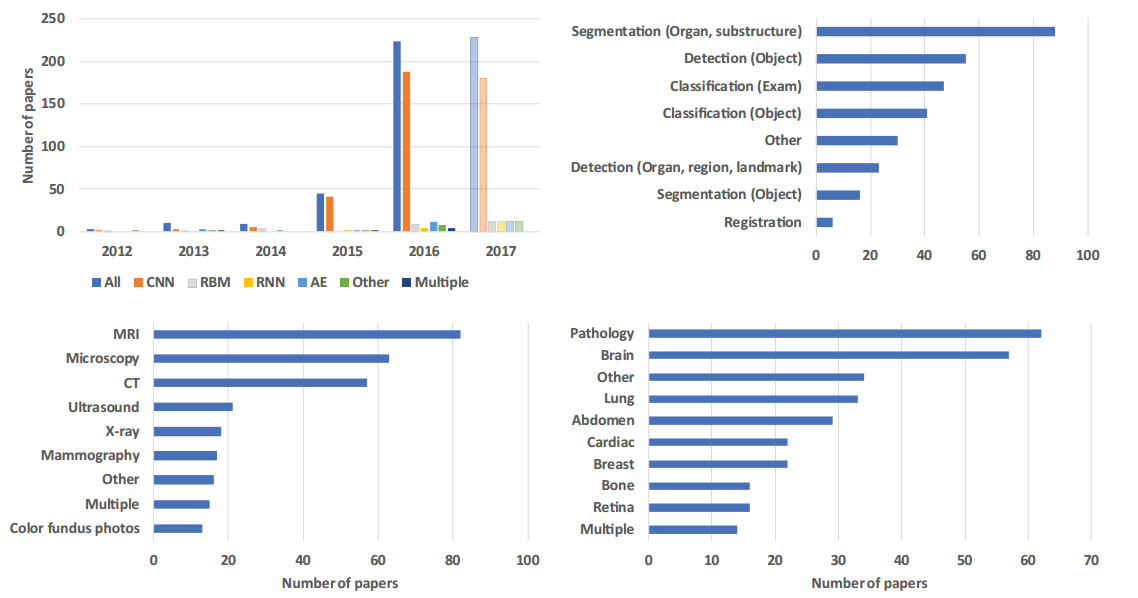
\includegraphics[width=\textwidth]{resources/1-1-num_papers.png}
    \caption{The recent statistics in publication of medical image analysis \cite{survey_on_medical_image_analysis}.}
    \label{fig:1-1-numpapers}
\end{figure}

Deep learning enables the computers to learn the features that are optimal to specific task. With the increasing amount of well-organized data in medical image analysis such as The Cancer Genome Atlas (TCGA) \cite{tcga}, there are gradually shifting attention from handcrafted approaches to deep learning. Figure \ref{fig:1-1-numpapers} visualizes the number of recently published papers in medical image analysis using deep learning in their proposed method. As can be seen in the graph, deep learning, especially convolutional neural networks (CNNs) \cite{AlexNet}, has become prominent approach in recent studies. CNNs are increasing the performance of a lot of tasks in medical image analysis. For example, in nuclear cell segmentation, the proposed CNN in \cite{he_dataset_kumar} improves the F1-score to about 83\% compared to 40\% of a configuration of handcrafted approaches. Not only the nuclear segmentation witnesses the increasing performance when deep learning is applied, the other areas such as disorder classification \cite{disorder1, disorder2}, abnormalities detection \cite{abnormality1, abnormality2}, also see this phenomenon. The anatomical application areas are also diverse, from brain \cite{brain}, eye \cite{eyes1, abnormality1}, chest \cite{chest1}, breast \cite{breast1} to digital pathology and microscopy \cite{he_dataset_kumar}. These mentioned examples is evidence that deep learning is really attracting great interest in the research community. 

\section{Motivation}

\subsection{The need of medical image analysis}

As mentioned in \cite{needofcellseg}, computer vision software, especially based on the latest deep learning algorithms, is enabling automated analysis medical image to provide accurate results that are delivered immeasurably faster than manual process can achieve. As these automated systems become pervasive in the healthcare industry, they may bring about radical changes in the way radiologists, clinicians, and even patients use imaging technology to monitor treatment and improve outcomes. Figure \ref{fig:1_2_deman_supply} shows a high demand of radiologists to consume the large a mount of images generated by our new technology such as CT or MRI tests. Developing new CADx systems brings immediate affects to our health care system, not just only shortening the amount of processed time but also increasing the accessibility to all of people, especially ones from remote areas. Besides the diagnosis help, the systems can also extract useful information for research purposes. Many laboratories around the world are conducting experiments such as on the living tissues to further investigate their properties to have better understanding of the insight mechanism or find better treatment. These aforementioned reasons are our motivation to do more research on the application of deep learning in medical image analysis, specifically nuclear segmentation \cite{G-U-Net}.

\begin{figure}
    \centering
    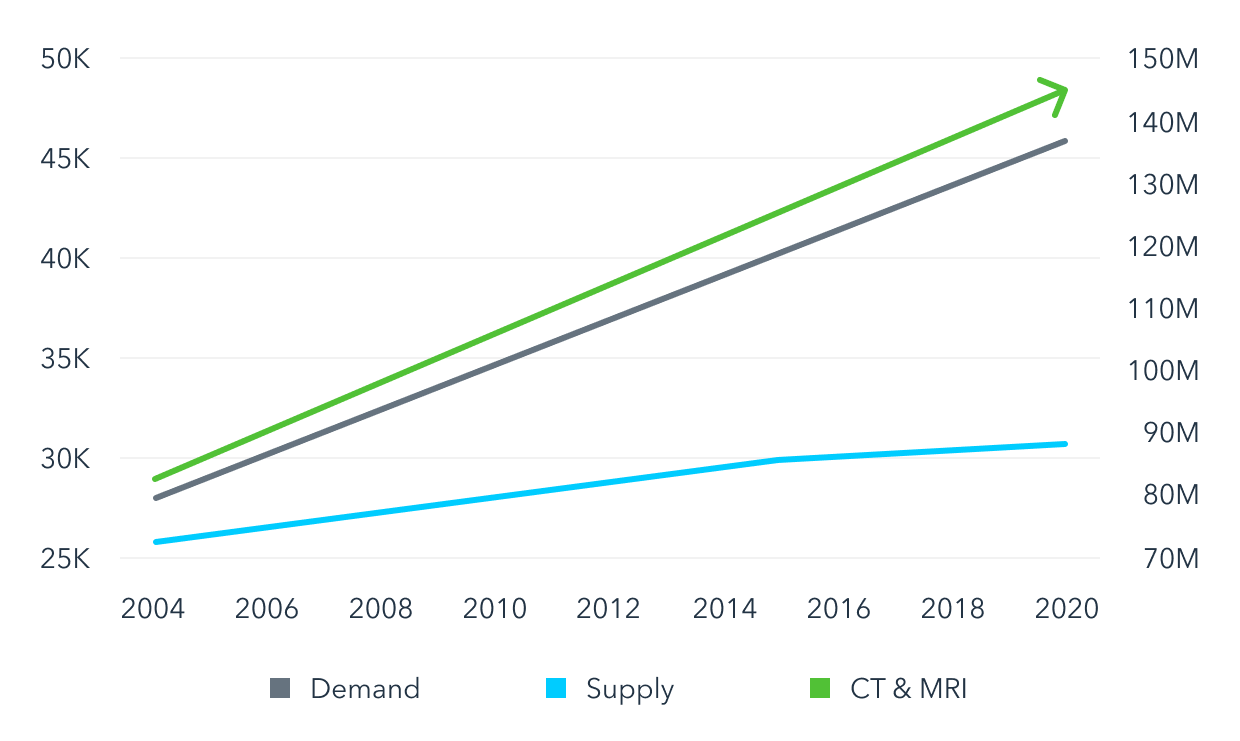
\includegraphics[width=0.8\textwidth]{resources/1-2-demand-and-supply-of-radiologists.png}
    \caption{Demand and supply of radiologists vs CT \& MRI tests \cite{needofcellseg}.}
    \label{fig:1_2_deman_supply}
\end{figure}


\subsection{Abnormality finding and landmark detection in endoscopic images}
Inspired from the fact that with the advances of computing technologies, multimedia communities together with computer scientists can involve in improving the healthcare system. The abnormality finding and landmark detection in endoscopy images challenge aim to bring new achievements in computer vision, image processing and machine learning to the next level of computer and multimedia assisted diagnosis. In details, these applications can solve a number of difficulties in processing images taking from medical devices. Currently, in order to take an endoscopy examination, patients have to pay a large amount of money and it takes them a lot of time. On the other hand, medical facilities can only handle a limit number of patient per day that can become a barrier for screening process on a 
large number of population.

Especially, new achievements in Biomedical Engineering has recently introduced a Wireless Capsule Device \cite{Moglia2007} that can be swallowed, and images can be captured automatically. Figure \ref{fig:capsule_device} shows images of that device. This device is convenient for patients that both cost and time for the examination are reduced. Besides, the willingness to undertake the examination also increased since they feel less discomfort. However, it is inconvenient for an endoscopist to watch 6-8 hours of videos. Instead, with the help of computer software system, selected images that contain special abnormal symptoms and anatomy landmarks and propose for a doctor automatically. 


\begin{figure}[thb]
	\centering 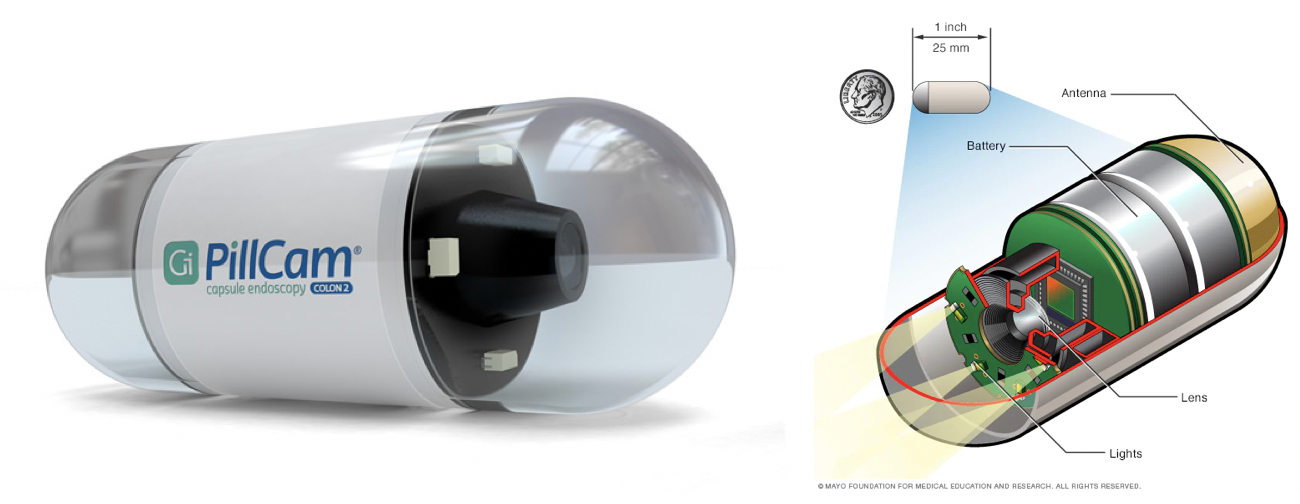
\includegraphics[width=0.9\columnwidth]{endoscopy_resources/capsule_endoscopy_img.png}
	\caption[Capsule endoscopy device.]{Capsule endoscopy device.\footnotemark.}
	\label{fig:capsule_device}
\end{figure}
\footnotetext{\url{www.mayoclinic.org/tests-procedures/capsule-endoscopy/about/pac-20393366} and
\url{www.tvgflorence.com/services-pillcam-capsule-endoscopy.html}}

In order to encourage the research community to tackle the problems with endoscopy images, several challenges had been conducted recently. For instance, the Medico: Multimedia Task at MediaEval 2018 challenge \cite{taskoverview} was successfully organized jointly with the MediaEval 2018 Workshop took place at EURECOM, Sophia Antipolis, France 29-31 October. Another workshop is going to be organized is the International Workshop on Multimedia for Personal Health and Health Care, which takes place in Nice, France, October 2019. The goal of these challenges is encouraging research communities to establish an assisted diagnosis systems that can detect abnormalities and anatomy landmarks in human gastrointestinal tract automatically. Some samples from the dataset proposed by both challenges are shown in Figure \ref{fig:gi_track_imgs}. Further information about these images and evaluation metric is given in Section \ref{dataset_evaluation_endoscopy}.

\begin{figure}[thb]
\begin{center}
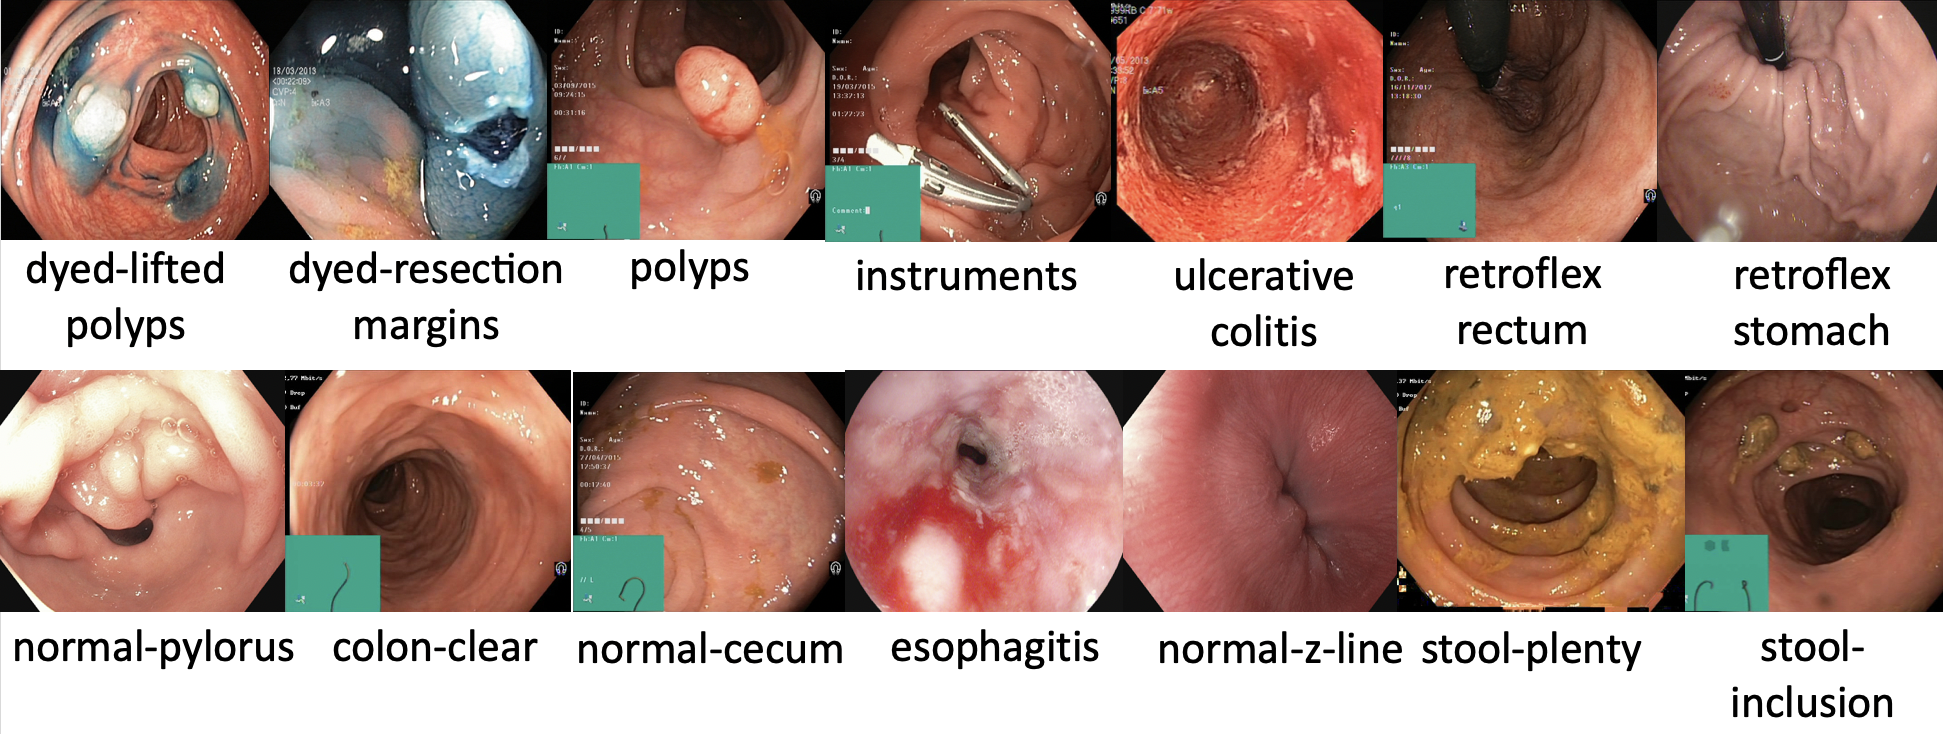
\includegraphics[width=\textwidth]{endoscopy_resources/gi_track_imgs.png}
\end{center}
  \caption {Abnormalities and anatomy landmarks in human gastrointestinal tract.}
\label{fig:gi_track_imgs}
\end{figure}


The task organizers also provide a priority list for the classes in other to accommodate with the single-class classification challenge. Thus, this leads to some modifications of our model, which are meticulously described in Section \ref{dataset_evaluation_endoscopy}.

In our approach, we introduce a stacked model consisting of two deep networks, a Residual Neural Network (ResNet) \cite{He_2016} followed by a Faster Region-based Convolutional Neural Network (Faster R-CNN) \cite{NIPS2015_5638}. 

Since ResNet mostly focuses on deep global features of image, it fails to classify images that symptoms of abnormal diseases or instruments appear as small objects on diversity backgrounds. Therefore, this is the reason of using Faster R-CNN to re-classify the images of some classes that Resnet usually mis-classify. Further information about our approaches is given in Section \ref{chap-method-endoscopy}.

\subsection{Nuclear segmentation problems in medical image analysis}

Nuclear segmentation in digital microscopic tissue images aims to separate individual nuclei and assign each pixel in image with a distinct index belonging to a single separated nuclei. As the motivation of Multi-organ Nuclei Segmentation Challenge 2018 (MoNuSeg 2018) \cite{monuseg} -  an official satellite event of the International Conference on Medical Image Computing \& Computer Assisted Intervention 2018 (MICCAI 2018), with accurately segmenting nuclei in diverse images spanning a range of patients, organs, and disease states, this can enable extraction of high-quality features for nuclear morphometrics, appearance features and other analysis in computational pathology such as density, nucleus-to-cytoplasm ratio, average size, pleomorphism, etc. These features can be used to assess not only cancer grades but also for predicting treatment effectiveness. Identifying different types of nuclei based on their segmentation can also yield information about gland shapes, which, for example, is important for cancer grading.

With mentioned challenges on the handcrafted approaches, deep learning shows significant improvements in medical image analysis, especially in nuclear segmentation. Although the amount of data in medical image analysis has increased dramatically during the deep learning era, such as the The Cancer Genome Atlas project (TCGA) \cite{tcga} with 2.5 petabytes of genomic, epigenomic, transcriptomic, and proteomic data, the number of annotated images are still limited because of the requirement of limited-time experts participating in labeling process. For example, a H\&E stained images dataset for nuclear segmentation proposed in \cite{he_dataset_kumar} containing only 30 images from TCGA project \cite{tcga} are considered as one of largest dataset in this filed. This is one of the our motivation to propose a new data augmentation process designed for histological images to synthetically increase the amount of training data, alleviating the effect of mentioned problem on training deep neural networks. Besides, the current segmentation architectures, for example UNet \cite{unet}, FCN \cite{FCNs}, also shown some limitations such as the missing of the equivariance to rotation group or the limited receptive field for separating touching nuclei task. The weakness of current design is also our motivation to propose new design to compensate the mentioned limitation, yielding the improvement in segmentation performance of the proposed architecture. The results of our proposed enhancements are discussed in more details in chapter \ref{chap-experiment}.


\section{Objectives}
% The Objective of our thesis is to propose enhancements for nuclear segmentation in H\&E histopathology images. The key idea of our proposed method is enforcing rotation equivariance in the network, the placement of residual blocks, and applying novel data augmentation designed specifically for these type of image. Our contribution to these enhancements includes:

The main objective of this thesis is to propose novel deep learning methods to improve the performance of deep learning approaches on medical image analysis systems which can assist experts in their daily job. Specifically, we are focusing on two main problems.  

\textit{Firstly}, in order to assist endoscopists, we propose enhancements for abnormality finding and anatomy landmark detection system on human gastrointestinal endoscopic images. The key idea of our proposed method is using a stacked model consisting of an image classification together with an object detection model. Besides, data augmentation takes an important role in training phase in order to overcome the limit number of training samples in medical dataset that can significant improve the overall performance. Our contribution to these enhancements includes:

\begin{enumerate}
    \item Propose additional information regarding to the abnormal positions of some special diseases that appear in the Kvasir dataset \cite{Pogorelov:2017:KMI:3083187.3083212}. 
    \item Propose a combination mechanism that can take advantages of both classification and object detection model on endoscopic images analysis.
    \item Propose an efficient data augmentation strategy on solving the imbalance between classes that happened in endoscopic image dataset. Moreover, it is also potential to be extended to solve these problems in similar situations.
\end{enumerate}

\textit{Secondly}, we propose enhancements for nuclear segmentation in H\&E histopathology images which can help pathologists during their diagnosis process. The key idea of our proposed method is enforcing rotation equivariance in the network, the placement of residual blocks, and applying novel data augmentation designed specifically for these type of image. Our contribution to these enhancements includes:

\begin{enumerate} [resume]
\item Encode equivariance to groups, specifically rotation and translation, following the work of group-equivariant CNNs (GCNNs) \cite{gcnn}, thereby obviating the need to learn such equivariance through extensive and time-consuming data augmentation.
\item Enhance the long-skip connections in the U-Net \cite{unet} from the downsampling to upsamling arms of the “U” with residual blocks \cite{Resnet}. 
\item Propose a novel means of data augmentation
specifically designed for histological images to aid in training.
\item Propose morphological post-processing method to yielding contiguous regions and accurate nuclear boundaries.
\end{enumerate} 


In order to fulfill our objective, in our thesis, we have to do the following tasks:
\begin{itemize}
\item Conduct researches on different abnormalities detection on medical image, from handcrafted approaches to deep learning approaches i.e Salient Superpixels \cite{bloodsalientsuperpixels}, color space approaches \cite{HSIColorDomain, active_blood_detect} etc. 

\item Conduct researches on different deep neural networks architecture for image classification and object detection tasks in Computer Vision such as InceptionNet \cite{inception}, DenseNet \cite{DenseNet}, ResNet \cite{Resnet}, YOLOv3 \cite{YOLOv3}, Fast R-CNN \cite{FastRCNN}, Faster R-CNN \cite{FasterRCNN},  etc.

\item Conduct researches on enhancing the performance of deep learning models with data augmentation mechanisms i.e Lucid Data Dreaming \cite{LucidDataDreaming_CVPR17_workshops}, GANs \cite{NIPS2014_5423}, etc.

\item Conduct experiments of our proposed enhancements and evaluate the results based on main score: Accuracy (ACC) and Matthews Correlation Coefficient (MCC) \cite{MATTHEWS1975442}.

\item Conduct researches on different nuclear segmentation not only on H\&E images but also in other related domains, i.e CNN3 \cite{he_dataset_kumar}, CNN2 \cite{cnn2}, Fiji \cite{fiji}, CellProfile \cite{cellprofile}, etc. 

\item Conduct researches on different deep neural networks architecture for segmentation tasks in Computer Vision such as AlexNet \cite{AlexNet}, VGG16 \cite{VGG16Net}, GoogleLeNet \cite{GoogleLeNet}, DenseNet \cite{DenseNet}, ResNet \cite{Resnet}, Feature Pyramid Network \cite{FPN}.

\item Conduct researches on enforcing rotation equivariance in the network, especially in convolutional neural networks, from GCNNs \cite{gcnn}, Cyclic Symmetry in CNNs \cite{cyclic_symmetry}, DREN \cite{dren}, P4M-DenseNet \cite{P4M-DenseNet}, etc.

\item Conduct researches on some semantic segmentation methods, especially instance segmentation, include UNet \cite{unet}, Mask R-CNN \cite{MaskRCNN}, MaskLab \cite{MaskLab}, PSPNet \cite{PSPNet}, FCNs \cite{FCNs}, DeepLab \cite{DeepLabv1,DeepLabv2,DeepLabv3,DeepLabv3+}.

\item Conduct experiments of our proposed enhancements with thoroughly designed ablation study and evaluate the results based on main score: Aggregated Jaccard Index \cite{he_dataset_kumar} (AJI).
\end{itemize}

\section{Thesis Content}
Our thesis is structured into 7 chapters:

\textbf{Chapter \ref{chap-introduction}} 

In chapter \ref{chap-introduction}, overview of recent developments of machine learning as well as deep learning in Computer Vision and their applications to conduct medical image analysis are represented. Classification, object detection together with segmentation are discussed in more details to indicate our motivations and objectives in this thesis. Besides, in this chapter, we also provide an overview of our thesis's structure.

\textbf{Chapter \ref{chap-related-works}}

In chapter \ref{chap-related-works}, methods used in several tasks in Computer Vision including image classification, object detection, object segmentation and instance segmentation are firstly discussed. We then describe recent approaches applied on abnormality finding in endoscopic image and nuclear segmentation problems in medical image analysis, in both handcrafted design and deep learning based methods. Additionally, we discuss about the recent development in incorporating group equivariance, especially rotation and translation groups in neural network.

\textbf{Chapter \ref{chap-method-endoscopy}}

In chapter \ref{chap-method-endoscopy}, we present our proposed method for abnormal finding and landmark detection in endoscopic images. Particularly, our proposed methods are used to take part in two challenges, including the Medico: The 2018 Multimedia for Medicine Task (Medico 2018) and The Biomedia ACM MM Grand Challenge 2019 (Biomedia 2019). Details about our approaches and improvements between two challenges are also reported. In sum, We utilize different  deep convolution neural network architectures together with several training techniques to improve the overall performance.


\textbf{Chapter \ref{chap-method}}

In this chapter, we present our proposed method for nuclear segmentation in H\&E stained histopathology images. Specifically, we consider enforcing rotation equivariance in the network, the placement of residual blocks, and applying novel data augmentation designed specifically for histopathology images, and show the relative improvement and merit of each. Incorporating all of these enhancements in the design and training of a U-Net yields significantly improved segmentation results while still maintaining a speed of inference that is sufficient for realworld applications, in particular, analyzing whole-slide images (WSIs).

\textbf{Chapter \ref{chap-experiment-endoscopy}}

In chapter \ref{chap-experiment-endoscopy}, we describe the dataset, task descriptions as well as the evaluation metrics used in both following challenges: The 2018 Multimedia for Medicine Task and and The Biomedia ACM MM Grand Challenge 2019. We not only report our official results provided by organizers but also discuss about the performance of each component in our algorithm by trying different experiment configurations and analyze the corresponding results.


\textbf{Chapter \ref{chap-experiment}}

In chapter \ref{chap-experiment}, we describe the Hematoxylin and Eosin (H\&E) stained histopathology images dataset taken from Multi-organ Nuclei Segmentation Challenge 2018 as well as the evaluation metrics we used to evaluate our proposed methods. We also discuss more about the results acquired in each step from our algorithm, which shows the merit of each component. Moreover, the ablation study are conducted to show the improvement of our proposed enhancements.

\textbf{Chapter \ref{chap-conclusion}}

In chapter \ref{chap-conclusion}, we re-declare the problem of abnormality finding and anatomical landmarks detection together with nuclear segmentation using deep convolution neural networks. Overview of what researches we conducted as well as analysis of future works are also discussed to provide the overall summary of our thesis. 

\begin{ChapAbstract}
%Computer scientists and medical scientists are very enthusiastic about their science. Recent developments of machine learning as well as deep learning in Computer Vision have improved human assisted diagnosis system. Classification, object detection together with segmentation are discussed in the context of medical images.   Besides, in this chapter, we also provide an overview of our thesis's structure.
\end{ChapAbstract}